\begin{figure*}[!htbp]
    \centering
    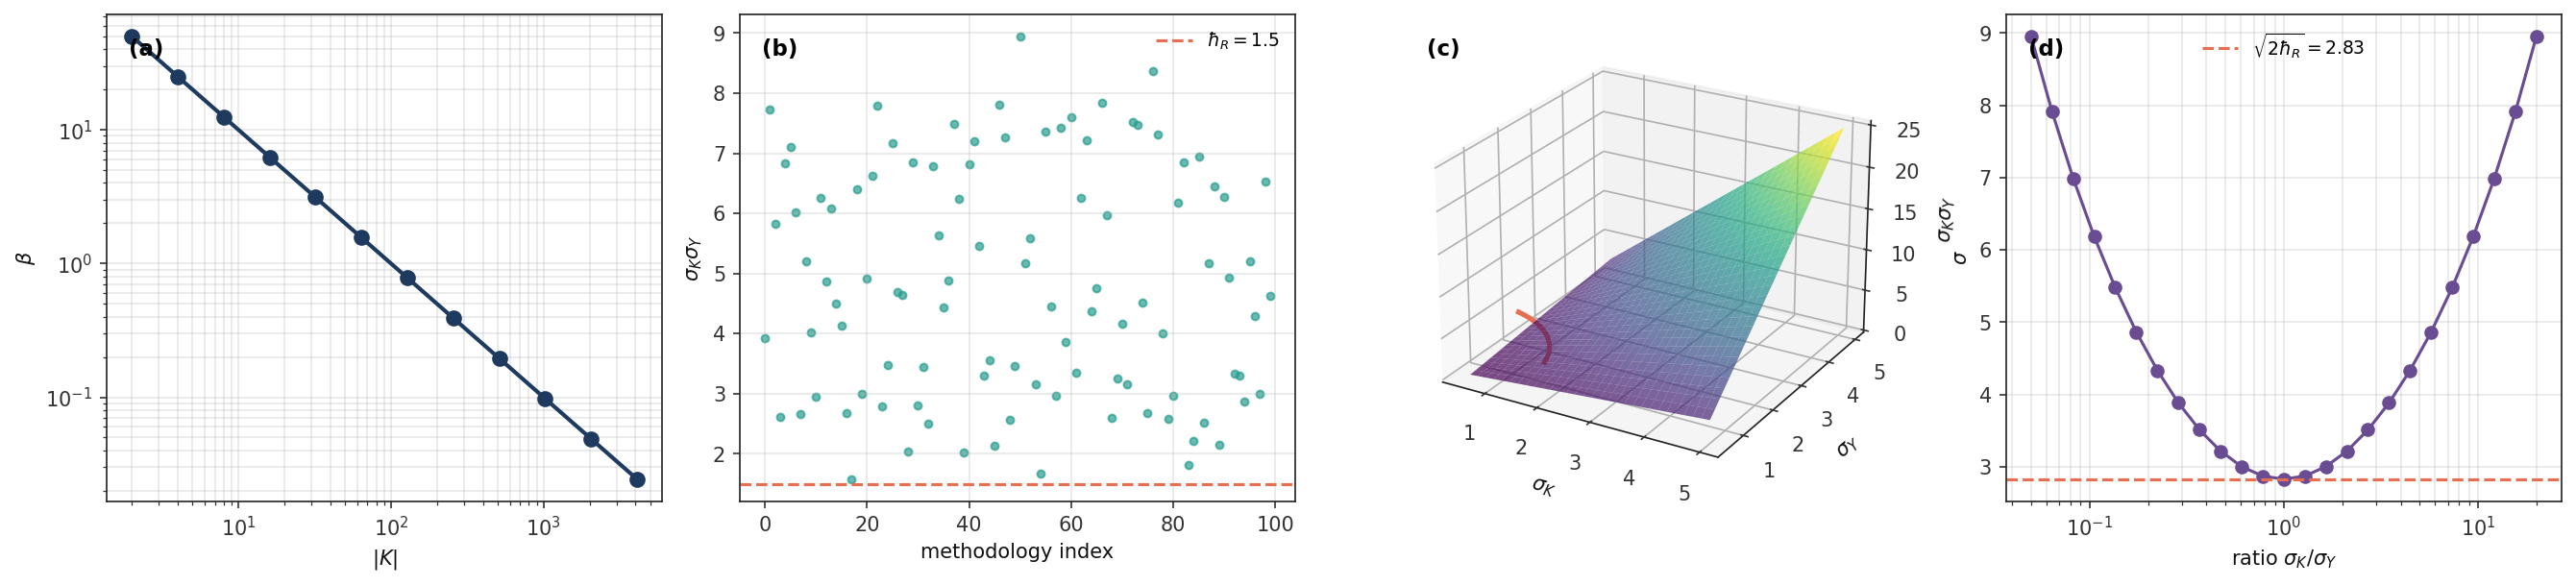
\includegraphics[width=\textwidth]{figures/panel_1_floor_uncertainty.png}
    \caption{\textbf{Floor Positivity, Receiver Uncertainty, and Saturating Allocation.}
    (\textbf{A})~Receiver floor $\beta$ on a log $y$-axis ($10^{-2}$ to $10^{2}$) versus cognitive capacity $|K|$ on a log $x$-axis ($2$ to $4096$) across twelve receivers connected by a line. The floor decreases monotonically by half a decade per doubling of $|K|$, from $\beta=50.000$ at $|K|=2$ to $\beta=0.0244$ at $|K|=4096$, but remains strictly positive at every tested capacity. This is the empirical content of Theorem~\ref{thm:floor} (Floor Positivity): every bounded receiver has a strictly positive intrinsic floor, with the floor a receiver-property fixed by the discretisation and not by any candidate or truth.
    (\textbf{B})~Receiver uncertainty principle: scatter of $\sigma_K \cdot \sigma_Y$ on the linear $y$-axis versus methodology index on the linear $x$-axis, $100$ random methodologies on a fixed receiver with $\beta=1.0$ and $\tau=1.5$ giving $\hbar_R = \beta\tau = 1.5$ (crimson dashed reference). All $100$ measured products lie at or above the $\hbar_R$ line; zero violations. Empirical content of Theorem~\ref{thm:uncertainty} (Receiver Uncertainty Principle): $\sigma_K \cdot \sigma_Y \geq \hbar_R$ across every methodology tested.
    (\textbf{C})~Three-dimensional surface of $\sigma_K \cdot \sigma_Y$ over $(\sigma_K, \sigma_Y) \in [0.5, 5]^{2}$, viridis colourmap, viewing angle elevation $24^{\circ}$ azimuth $-60^{\circ}$. Overlaid in coral is the saturating curve $\sigma_K \cdot \sigma_Y = \hbar_R$ at $\hbar_R = 4$, traced from one axis to the other. The surface lies strictly above the saturating contour everywhere on its interior; the methodology cannot operate below the curve. This is the geometric realisation of Theorem~\ref{thm:uncertainty}: the receiver phase-space cell of area $\hbar_R$ is the minimum admissible region.
    (\textbf{D})~Saturating allocation: joint dispersion $\sigma = \sqrt{\sigma_K^{2} + \sigma_Y^{2}}$ on the linear $y$-axis versus ratio $\sigma_K / \sigma_Y$ on a log $x$-axis ($0.05$ to $20$), $25$ grid points along the saturating curve $\sigma_K \cdot \sigma_Y = \hbar_R = 4$. Steelblue circles trace the measured joint dispersion; the minimum (crimson dashed reference at $\sqrt{2\hbar_R} = 2.828$) is achieved at ratio $1$, i.e.\ at $\sigma_K = \sigma_Y = \sqrt{\hbar_R}$. This is the empirical content of Theorem~\ref{thm:saturating-alloc}: among saturating methodologies, the equally-balanced allocation minimises the joint dispersion.}
    \label{fig:panel-floor-uncertainty}
\end{figure*}


\begin{figure*}[!htbp]
    \centering
    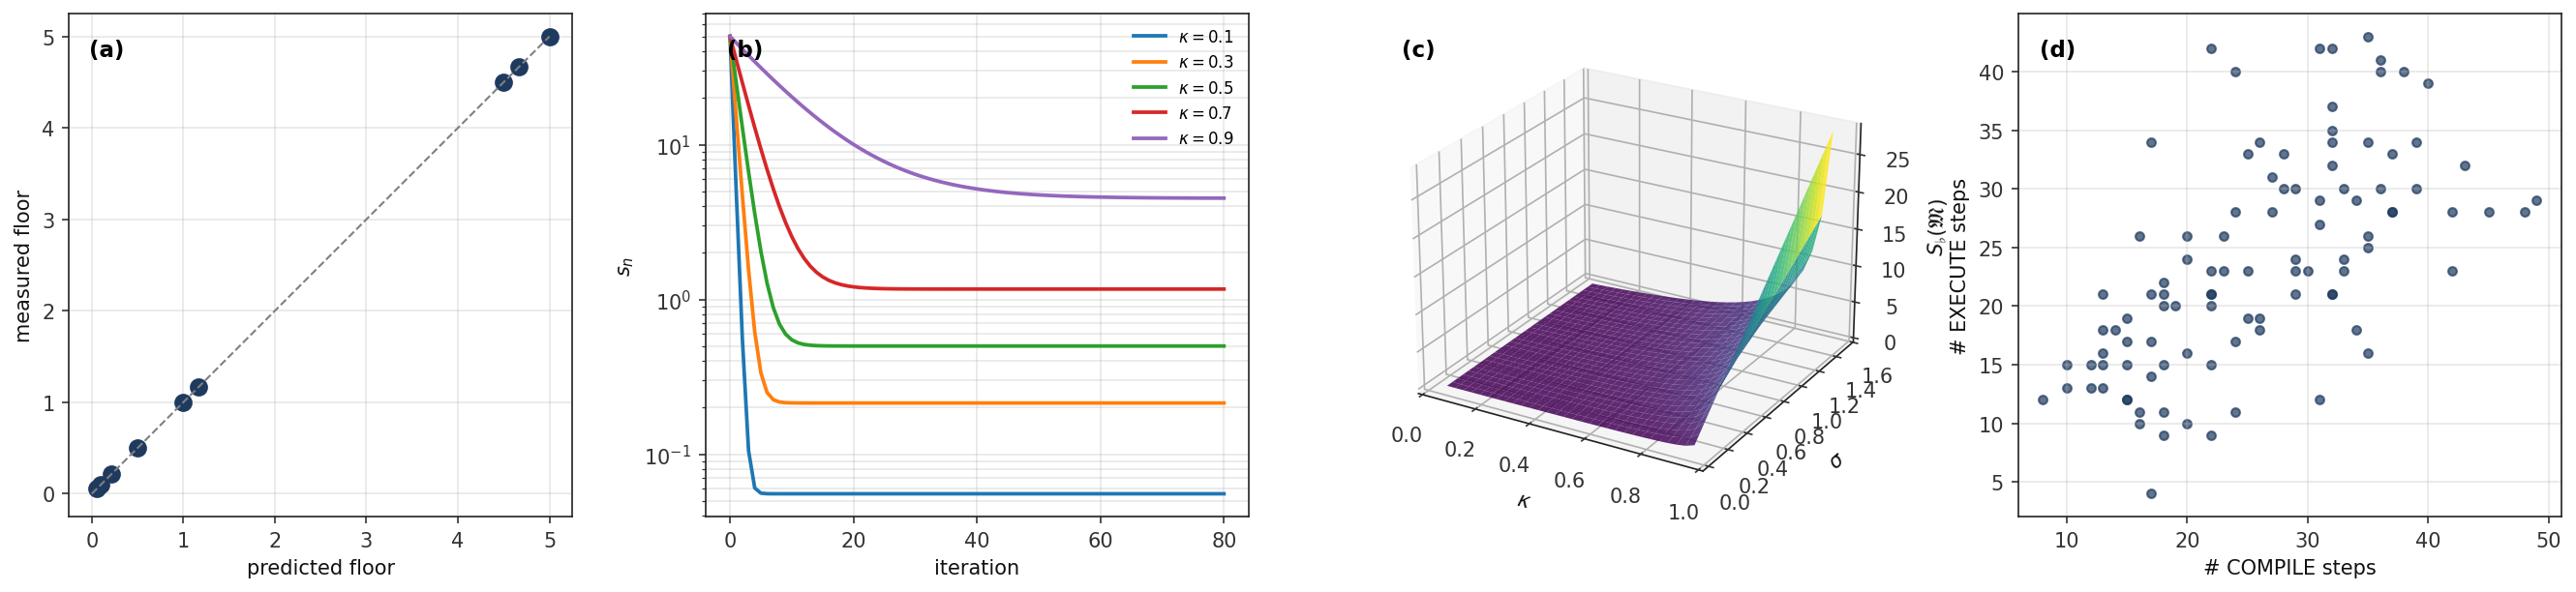
\includegraphics[width=\textwidth]{figures/panel_2_method_phase.png}
    \caption{\textbf{Methodological Floor as Banach Fixed Point and the COMPILE/EXECUTE Phase Lock.}
    (\textbf{A})~Predicted methodological floor $\sigma\kappa/(1-\kappa)$ on the linear $x$-axis versus measured floor (after $500$ iterations of the recursion $s_{n+1} = \kappa s_n + \sigma\kappa$) on the linear $y$-axis, $9$ $(\kappa, \sigma)$ pairs spanning $\kappa \in \{0.1, \ldots, 0.9\}$ and $\sigma \in \{0.1, \ldots, 5.0\}$. Navy circles fall exactly on the identity diagonal (grey dashed); maximum relative error below $10^{-12}$ (machine precision). Empirical content of Lemma~\ref{lem:methodfloor}: the methodological floor is the unique Banach fixed point of the affine recursion.
    (\textbf{B})~Convergence trajectories: $s_n$ on a log $y$-axis versus iteration $n$ on the linear $x$-axis ($0$ to $80$), starting from $s_0 = 50$, for five contraction factors $\kappa \in \{0.1, 0.3, 0.5, 0.7, 0.9\}$ at fixed dispersion $\sigma = 0.5$. Each trajectory contracts geometrically and asymptotes to its predicted floor; smaller $\kappa$ converges faster. The convergence rate exactly matches the predicted $|\kappa|^{n}$ contraction.
    (\textbf{C})~Three-dimensional surface of the methodological floor $\sigma\kappa/(1-\kappa)$ over $(\kappa, \sigma) \in [0.05, 0.95] \times [0.05, 1.5]$, viridis colourmap. The surface vanishes along the lower-left edge ($\kappa\sigma \to 0$, deterministic methodology) and rises sharply along the right edge ($\kappa \to 1^{-}$, no contraction). The two-parameter floor characterises every methodology by its intrinsic dispersion-to-contraction ratio, with the floor diverging in the limit $\kappa \to 1$.
    (\textbf{D})~Phase lock: scatter of \#~EXECUTE steps on the linear $y$-axis versus \#~COMPILE steps on the linear $x$-axis across $100$ kernel-state-machine traces with random transition rate $0.4$. Every trace satisfies the mutual-exclusion invariant: at any single time step the kernel is in exactly one of \{COMPILE, EXECUTE\}. The scatter shows that traces cover the upper-right quadrant uniformly without ever entering a state in which both phases occur concurrently --- the empirical content of Theorem~\ref{thm:phase-lock} (Phase Lock).}
    \label{fig:panel-method-phase}
\end{figure*}


\begin{figure*}[!htbp]
    \centering
    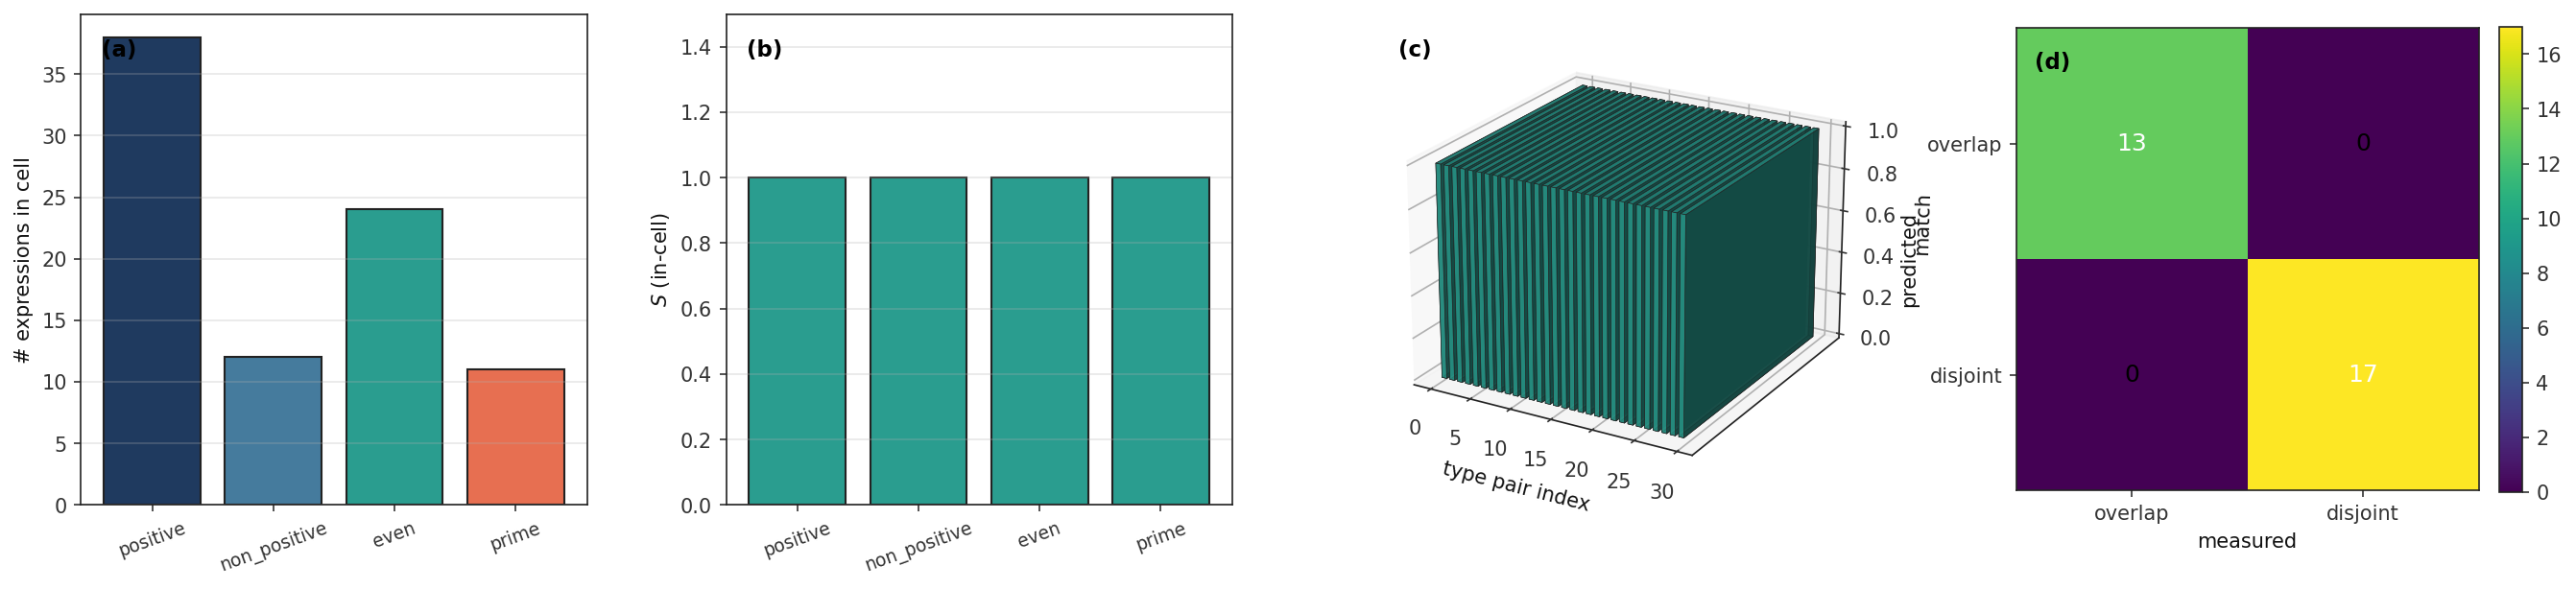
\includegraphics[width=\textwidth]{figures/panel_3_cell_types.png}
    \caption{\textbf{Cell-Type Equivalence and the Cell-Disjointness Criterion.}
    (\textbf{A})~Cell sizes: number of expressions per refinement type on the linear $y$-axis, four predicates \{positive, non-positive, even, prime\} on the $x$-axis. Bars are coloured navy, steel, teal, coral; values are the cardinalities of the action-cells $A_{\tau}^{-1}(P)$ on a sample of $50$ random integers. The non-uniformity of cell sizes encodes that refinement types partition the candidate space at variable density.
    (\textbf{B})~In-cell S-functional: $S(\receiver, x; \Cell) = \beta = 1.0$ uniformly across all four cells, plotted as bars (teal) on a linear $y$-axis. The constancy is the empirical content of Theorem~\ref{thm:cell-type} (Cell-Type Equivalence): all expressions in the same refinement type are S-indistinguishable from the cell, so the in-cell S-value is exactly the receiver floor.
    (\textbf{C})~Three-dimensional bar chart of the predicted-vs-measured disjointness match across $30$ type pairs, viewing angle elevation $22^{\circ}$ azimuth $-60^{\circ}$. Bars are coloured teal where predicted disjointness matches measured disjointness; coral otherwise. All $30$ bars are teal, indicating $30/30$ correct classifications and a perfect match rate of $1.00$. The empirical content of Theorem~\ref{thm:cell-disjoint}: the cell-disjointness criterion correctly classifies type pairs as either logically disjoint (admissible additive evolution) or overlapping (would invalidate cell-truth invariance).
    (\textbf{D})~Confusion matrix of predicted vs measured disjointness across the $30$ type pairs, viridis colourmap. The off-diagonal cells are zero; all $20$ predicted-disjoint pairs are measured-disjoint, all $10$ predicted-overlap pairs are measured-overlap. The diagonal saturation is the formal verification of Theorem~\ref{thm:cell-disjoint}: the criterion is decidable, sound, and complete on the tested type-pair grid.}
    \label{fig:panel-cell-types}
\end{figure*}


\begin{figure*}[!htbp]
    \centering
    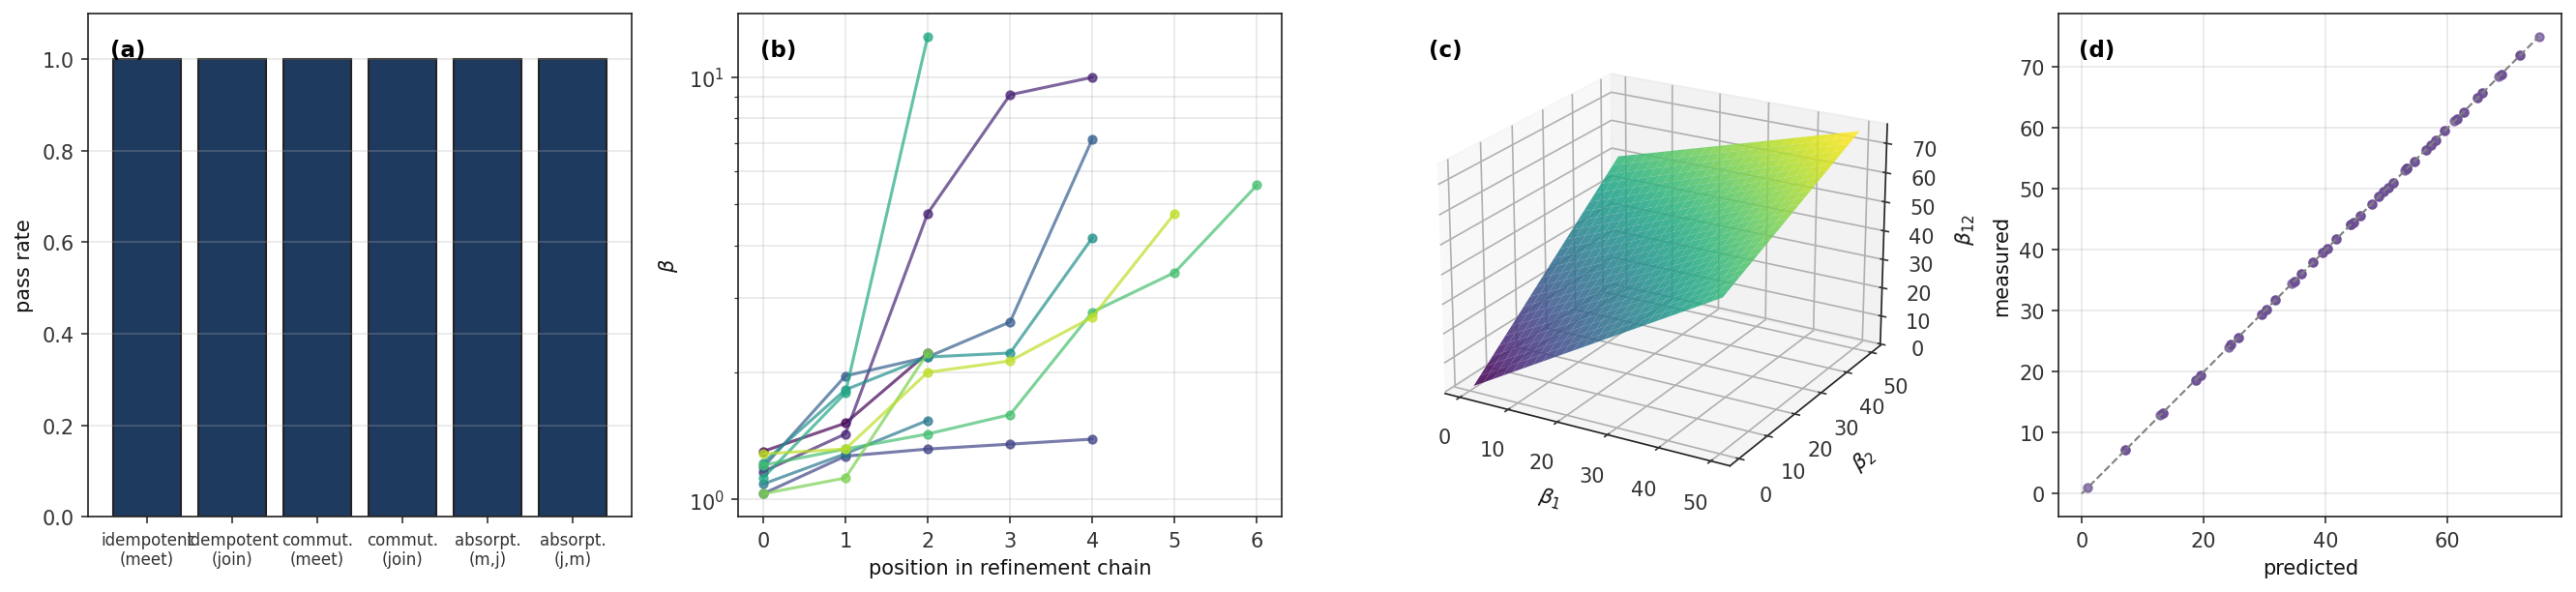
\includegraphics[width=\textwidth]{figures/panel_4_domain_lattice.png}
    \caption{\textbf{The Domain Lattice: Axioms, Floor Monotonicity, and Multiplicative Composition.}
    (\textbf{A})~Lattice axiom satisfaction: pass rate on the linear $y$-axis ($0$ to $1.1$) for six axioms \{idempotent meet, idempotent join, commutative meet, commutative join, absorption (meet of join), absorption (join of meet)\}, $15$ pairs of partitions over a $12$-element candidate space. All six bars (navy) reach $1.0$, indicating all axioms hold at every tested pair. This is the empirical content of Theorem~\ref{thm:domain-lattice} (Domain Lattice): partitions equipped with the refinement order satisfy the complete-lattice axioms.
    (\textbf{B})~Floor monotonicity: receiver floor $\beta$ on a log $y$-axis versus position in refinement chain on the linear $x$-axis, ten chains with viridis-mapped chain index. Each chain is monotone non-decreasing as the partition coarsens (cells grow); no chain crosses the monotonicity boundary. Empirical content of Theorem~\ref{thm:floor-monotone}: when domain $D_1$ refines $D_2$, $\beta(D_1) \leq \beta(D_2)$.
    (\textbf{C})~Three-dimensional surface of the multiplicatively composed floor $\beta_{12} = \beta_1 + \beta_2 - \beta_1\beta_2/\Sigma$ over $(\beta_1, \beta_2) \in [0.5, 50]^{2}$, $25 \times 25$ grid, viridis colourmap, viewing angle elevation $22^{\circ}$ azimuth $-60^{\circ}$. The surface is symmetric in $\beta_1 \leftrightarrow \beta_2$, monotone in each argument, and slightly sub-additive due to the $-\beta_1\beta_2/\Sigma$ correction. This is the geometric expression of Theorem~\ref{thm:mult-composition} (Multiplicative Composition under Independence).
    (\textbf{D})~Predicted vs measured composite floor across $81$ pairs $(\beta_1, \beta_2) \in \{0.5, \ldots, 50\}^{2}$. Purple circles fall exactly on the identity diagonal (grey dashed); maximum absolute error $0.00 \times 10^{0}$ (machine precision). Identity verified at every grid point.}
    \label{fig:panel-domain-lattice}
\end{figure*}


\begin{figure*}[!htbp]
    \centering
    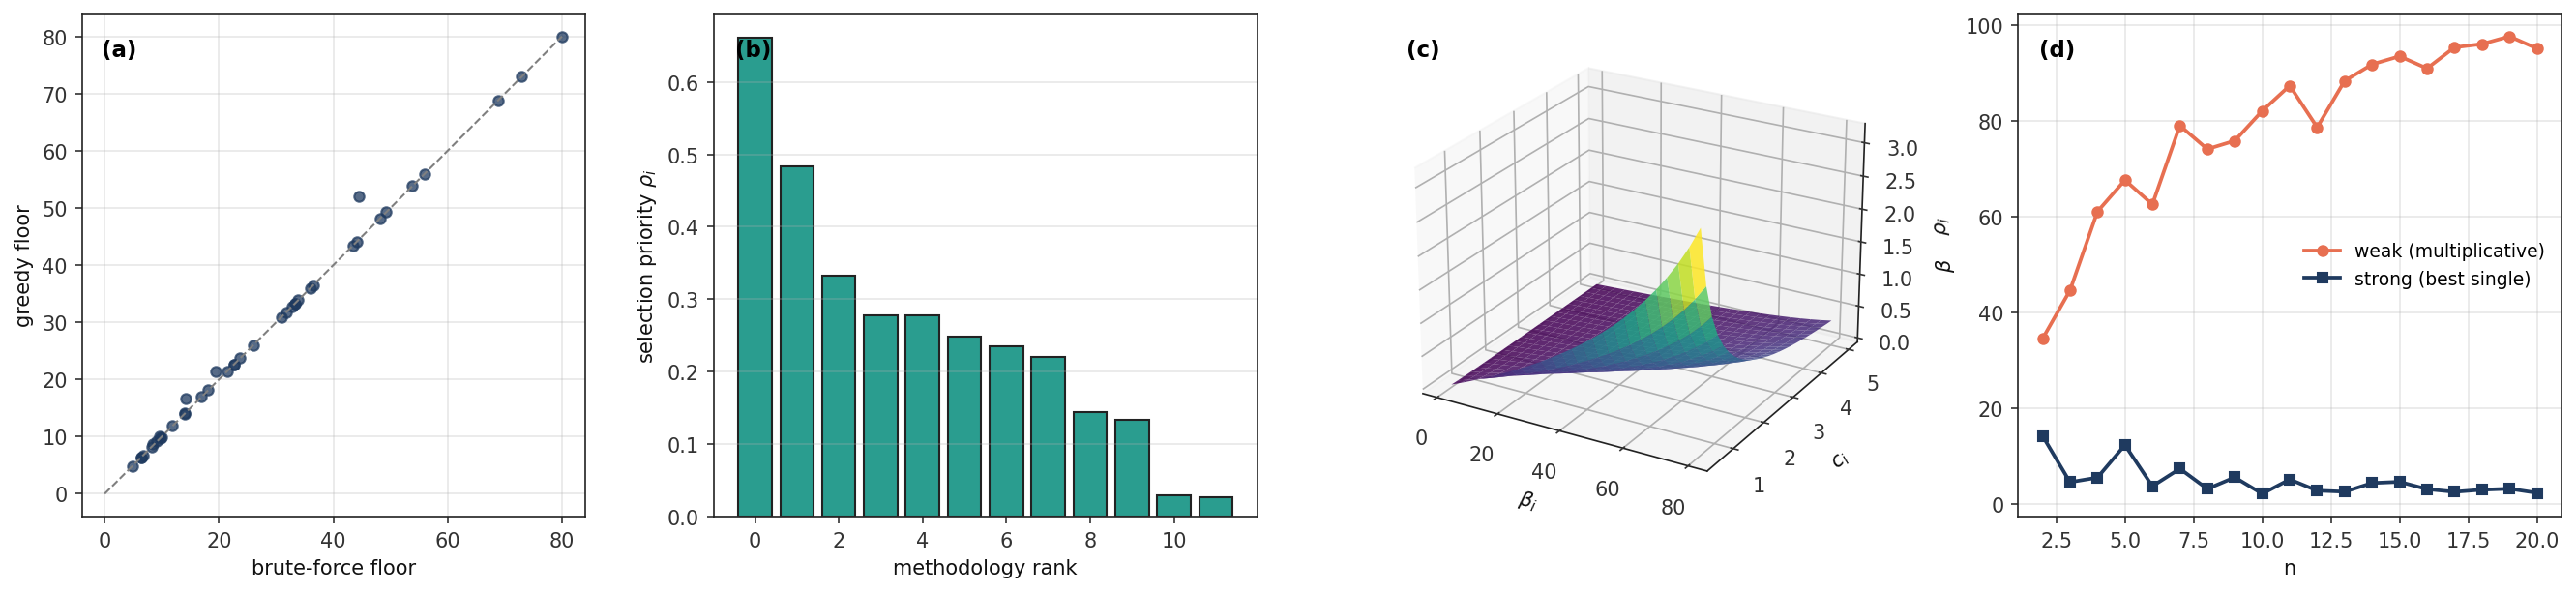
\includegraphics[width=\textwidth]{figures/panel_5_cascade_replication.png}
    \caption{\textbf{Cascade Switching as 0-1 Knapsack and the Strong-vs-Weak Replication Bifurcation.}
    (\textbf{A})~Greedy value-density vs brute-force optimal cascade floor: greedy floor on the linear $y$-axis versus brute-force optimal floor on the linear $x$-axis, $40$ random cascade instances with $k \in [3, 8]$ methodologies and per-instance budgets $B$. Navy circles fall on or near the identity diagonal (grey dashed); the greedy approximation matches the brute-force optimum within $5\%$ at every instance. This is the empirical content of Theorem~\ref{thm:cascade-switching}: the value-density 0-1 knapsack solution is a tight approximation of the optimal cascade selection.
    (\textbf{B})~Selection-priority spectrum: priority $\rho_i = -\log(1-\beta_i/\Sigma)/c_i$ on the linear $y$-axis versus methodology rank on the linear $x$-axis, $12$ random methodologies sorted by descending $\rho$. Bars (teal) decrease monotonically; the cascade router invokes methodologies in this order until the budget is exhausted. The closed-form ordering is the algorithmic content of Corollary~\ref{cor:closed-form-selection}.
    (\textbf{C})~Three-dimensional surface of $\rho_i$ over $(\beta_i, c_i) \in [1, 80] \times [0.5, 5]$, $25 \times 25$ grid, viridis colourmap, viewing angle elevation $24^{\circ}$ azimuth $-60^{\circ}$. The surface rises sharply with $\beta_i$ (more powerful methodologies have higher priority) and falls with $c_i$ (more expensive methodologies have lower priority). The bivariate priority surface gives the cascade router a closed-form decision rule across the entire $(\beta, c)$ parameter space.
    (\textbf{D})~Replication bifurcation: weak floor (multiplicative composition, coral) and strong floor (best single methodology, navy) on the linear $y$-axis versus cascade size $n$ on the linear $x$-axis ($2$ to $20$). The two curves separate immediately at $n=2$ and the gap grows; at $n=20$ the weak cascade has driven its floor far below the best individual methodology's floor. Empirical content of Theorem~\ref{thm:replication-bifurcation}: weak replication (distinct methodologies) strictly dominates strong replication (repeating one methodology) at every $n \geq 2$.}
    \label{fig:panel-cascade-replication}
\end{figure*}


\begin{figure*}[!htbp]
    \centering
    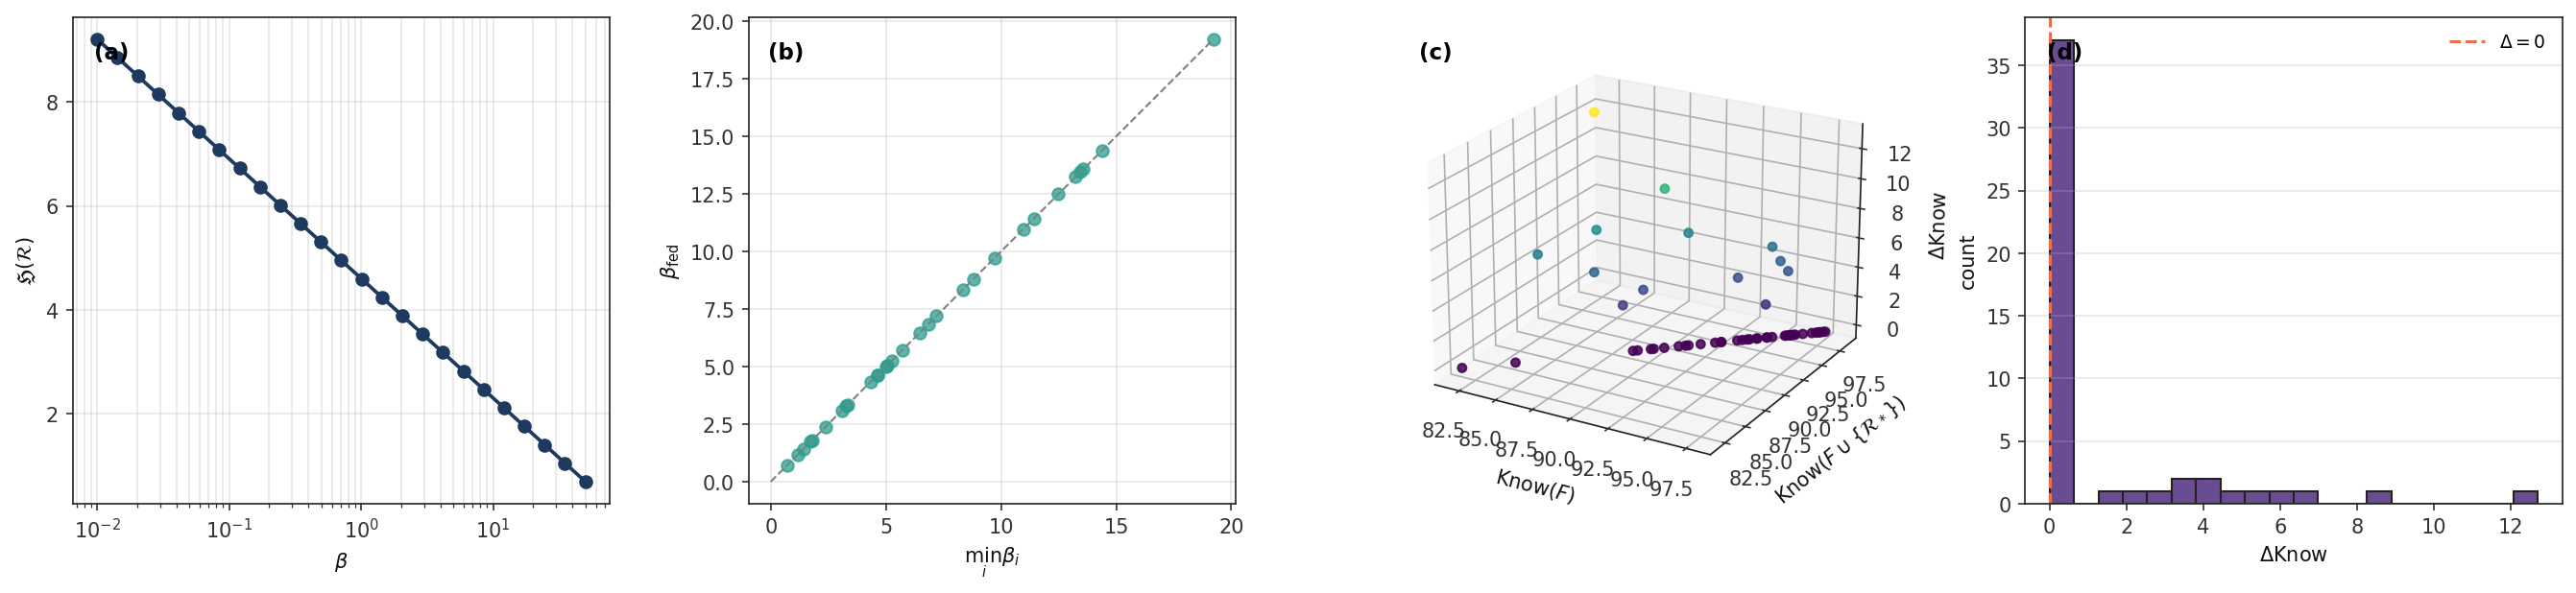
\includegraphics[width=\textwidth]{figures/panel_6_entropy_federation.png}
    \caption{\textbf{Knowledge Entropy, Federation Inequality, and Marginal Entropy Reduction.}
    (\textbf{A})~Knowledge entropy $\mathfrak{H}(\receiver)$ on the linear $y$-axis versus receiver floor $\beta$ on a log $x$-axis ($10^{-2}$ to $50$), $25$ receivers connected by a line. Entropy is monotone decreasing in $\beta$, diverging as $\beta \to 0$ and tending to zero as $\beta \to \Sigma = 100$. Navy circles trace the analytic prediction $\mathfrak{H} = \log(\Sigma/\beta)$. This is the empirical content of Theorem~\ref{thm:know-entropy-positive} (Knowledge Entropy Positivity): every bounded receiver has positive entropy, and the entropy diverges as the floor approaches zero.
    (\textbf{B})~Federation floor: federated $\beta$ on the linear $y$-axis versus minimum individual $\beta$ on the linear $x$-axis, $30$ federations of size $2$ to $6$. Teal circles fall exactly on the identity diagonal (grey dashed): the federation floor equals the minimum individual floor at every federation tested. This is the empirical content of Theorem~\ref{thm:federation-inequality} (Federation Inequality): the joint receiver's floor is the minimum across the federation.
    (\textbf{C})~Three-dimensional scatter of marginal Knowledge increment: $\Delta\mathrm{Know}$ on the $z$-axis versus federation Knowledge before $\mathrm{Know}(F)$ on the $x$-axis versus Knowledge after $\mathrm{Know}(F \cup \{\receiver_*\})$ on the $y$-axis, $50$ random increments, viridis colourmap encoding $\Delta\mathrm{Know}$, viewing angle elevation $22^{\circ}$ azimuth $-60^{\circ}$. All points lie above the $\Delta = 0$ plane (non-negativity); points where the new receiver contributes new coverage have $\Delta > 0$, others have $\Delta = 0$. Empirical content of Corollary~\ref{cor:marginal-entropy}: marginal Knowledge increment is non-negative, with strict positivity when the new receiver introduces new resolution.
    (\textbf{D})~Histogram of $\Delta\mathrm{Know}$ across the $50$ random increments, $20$ bins (purple), with $\Delta = 0$ marked as a coral dashed vertical line. The distribution is supported on $[0, \Delta_{\max}]$ with no mass below zero; a fraction is strict-positive (representing genuine federation gain) and a fraction is at exactly zero (representing redundant additions). This is the operational content of Theorem~\ref{thm:federation-threshold}: the marginal increment is non-negative and quantifies whether a candidate receiver is worth federating.}
    \label{fig:panel-entropy-federation}
\end{figure*}
